\documentclass[a4paper,10pt]{ltjsarticle}
\usepackage[top=11mm,bottom=10mm,left=16mm,right=16mm]{geometry}
\usepackage{amsmath,amssymb}
\usepackage{xcolor}
\usepackage{tikz}
\usetikzlibrary{calc}
\usepackage[most]{tcolorbox}

% ---- フォントは指定せず，ltjsarticle の既定（自動選択）に任せる ----
% 和文ゴシックは \gtfamily で切り替え可能（明朝は既定 \mcfamily）

% ---- Palette ----
\definecolor{ink}{HTML}{1F3A5F}      % deep indigo
\definecolor{inklt}{HTML}{3E6398}
\definecolor{tint}{HTML}{EEF3F9}     % pale panel
\definecolor{tint2}{HTML}{E3ECF6}
\definecolor{gold}{HTML}{B07A2E}     % warm accent
\definecolor{rule}{HTML}{C9D6E5}
\definecolor{paper}{HTML}{FBFCFE}

\pagecolor{paper}
\color{ink!92!black}

% ---- Display spacing (compact but airy) ----
\setlength{\abovedisplayskip}{3pt}
\setlength{\belowdisplayskip}{3pt}
\setlength{\abovedisplayshortskip}{1.5pt}
\setlength{\belowdisplayshortskip}{2pt}
\setlength{\parindent}{0pt}
\linespread{1.0}

% ---- Step heading: numbered badge + gothic title ----
\newcounter{stepc}
\newcommand{\step}[1]{%
  \refstepcounter{stepc}%
  \vspace{1pt}%
  \noindent
  
\begin{tikzpicture}[baseline=(b.base)]
    \node[circle, fill=ink, text=white, inner sep=0pt, minimum size=6.2mm,
          font=\bfseries] (b) {\thestepc};
  \end{tikzpicture}%
  \hspace{5pt}\raisebox{1.1mm}{\gtfamily\bfseries\large\color{ink}#1}\par
  \vspace{-1pt}%
  {\color{rule}\rule{\linewidth}{0.9pt}}\par
  \vspace{1pt}%
}

\begin{document}

% ============ HEADER ============
\noindent
\begin{tikzpicture}
  \node[anchor=west,inner sep=0pt] (t) at (0,0)
     {\gtfamily\bfseries\fontsize{22}{22}\selectfont\color{ink}四面体の体積};
\end{tikzpicture}\\[1pt]
{\color{gold}\rule{\linewidth}{1.6pt}}
\vspace{2pt}

% ============ PROBLEM + FIGURE ============
\begin{tcolorbox}[enhanced, sharp corners=south, colback=tint, colframe=ink,
  boxrule=0pt, leftrule=3pt, top=5pt, bottom=6pt, left=10pt, right=10pt,
  overlay={\fill[ink] (frame.north west) rectangle ($(frame.north east)+(0,-6.6mm)$);
           \node[anchor=west, text=white, font=\gtfamily\bfseries]
             at ($(frame.north west)+(3.5mm,-3.3mm)$) {問\, 題};},
  before upper={\vspace{6.0mm}}]
\begin{minipage}[c]{0.60\linewidth}
$O(0,0,0)$，$A(6,0,-2)$，$B(0,6,3)$，$C(5,-1,6)$ を $4$ つの頂点とする
四面体の体積 $V$ を求めよ。
\end{minipage}\hfill
\begin{minipage}[c]{0.36\linewidth}\centering
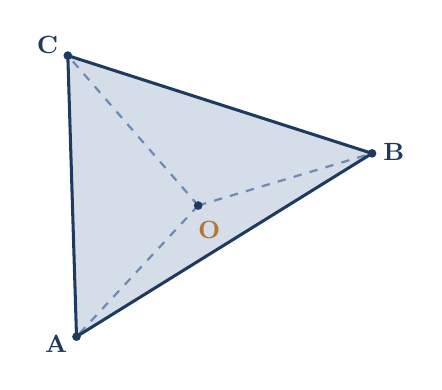
\begin{tikzpicture}[scale=0.92, line join=round]
  \coordinate (O) at (-0.30,-0.13);
  \coordinate (A) at (-1.98,-1.94);
  \coordinate (B) at ( 2.10, 0.59);
  \coordinate (C) at (-2.10, 1.94);
  % base face ABC (front)
  \fill[inklt!22] (A)--(B)--(C)--cycle;
  % hidden edges to back apex O (dashed)
  \draw[inklt!75, dashed, line width=0.8pt] (O)--(A);
  \draw[inklt!75, dashed, line width=0.8pt] (O)--(B);
  \draw[inklt!75, dashed, line width=0.8pt] (O)--(C);
  % front face edges (solid)
  \draw[ink, line width=1.1pt] (A)--(B)--(C)--cycle;
  % vertices
  \foreach \p in {O,A,B,C}{\fill[ink] (\p) circle (1.7pt);}
  \node[gold,font=\bfseries\small] at ($(O)+(0.15,-0.34)$) {O};
  \node[ink, font=\bfseries\small] at ($(A)+(-0.28,-0.10)$) {A};
  \node[ink, font=\bfseries\small] at ($(B)+(0.30,0.02)$)  {B};
  \node[ink, font=\bfseries\small] at ($(C)+(-0.28,0.14)$) {C};
\end{tikzpicture}
\end{minipage}
\end{tcolorbox}

\begin{center}

\fbox{\noindent\textbf{\gtfamily 方針}\;\;三角形 $ABC$ を底面とみなし，点 $O$ から平面 $ABC$ までの距離を高さとして体積を求める。}

\end{center}

% ============ STEPS ============
\step{ベクトルの準備}
辺ベクトルとその長さ・内積を求める。
\[
\overrightarrow{AB}=B-A=(-6,6,5),\qquad
\overrightarrow{AC}=C-A=(-1,-1,8),
\]
\[
|\overrightarrow{AB}|=\sqrt{36+36+25}=\sqrt{97},\quad
|\overrightarrow{AC}|=\sqrt{1+1+64}=\sqrt{66},\quad
\overrightarrow{AB}\cdot\overrightarrow{AC}=6-6+40=40.
\]

\step{底面 $\triangle ABC$ の面積 $S$}
$\cos\angle BAC=\dfrac{40}{\sqrt{97}\sqrt{66}}$ と公式$\cos^2+\sin^2=1$より $\sin\angle BAC=\dfrac{\sqrt{97\cdot66-40^{2}}}{\sqrt{97}\sqrt{66}}$．よって
\[
S=\tfrac12\,|\overrightarrow{AB}|\,|\overrightarrow{AC}|\sin\angle BAC
 =\frac{\sqrt{97\cdot66-1600}}{2}
 =\frac{\sqrt{4802}}{2}
 =\frac{49\sqrt{2}}{2}.
\]

\step{平面 $ABC$ の方程式}
$ABC$ に垂直なベクトルを, 長さは何でもいいので $\vec n=(p,q,1)$ とおくと，$\vec n\perp\overrightarrow{AB},\ \vec n\perp\overrightarrow{AC}$ より
\[
-6p+6q+5=0,\qquad -p-q+8=0
\ \Longrightarrow\ 43p=53q,\quad (p,q)=\Bigl(\tfrac{53}{12},\tfrac{43}{12}\Bigr).
\]
平面 $ABC$上の点$P(x,y,z)$は、 $\overrightarrow{AP}=(x-6,y,z+2)$が$12\vec n=(53, 43, 12)$に垂直になるので、平面 $ABC$ の方程式は、
\[
53(x-6)+43y+12(z+2)=0
\quad\Longrightarrow\quad
53x+43y+12z-294=0.
\]

\step{点 $O$ と平面の距離 $h$}
点 $Q(x_0,y_0,z_0)$ と平面 $ax+by+cz+d=0$ の距離は $\dfrac{|ax_0+by_0+cz_0+d|}{\sqrt{a^2+b^2+c^2}}$ で与えられる。$Q=(0,0,0)$ を代入して
\[
h=\frac{|-294|}{\sqrt{53^{2}+43^{2}+12^{2}}}
 =\frac{294}{\sqrt{4802}}
 =\frac{294}{49\sqrt{2}}
 =3\sqrt{2}.
\]

\step{体積の計算}
底面積 $S$ と高さ $h$ から，四面体の体積は
\[
V=\frac13\,S\,h
 =\frac13\cdot\frac{49\sqrt{2}}{2}\cdot 3\sqrt{2}
 =\frac13\cdot 147
 =49.
\]

% ============ ANSWER ============
\vspace{0pt}
\begin{center}
\begin{tcolorbox}[enhanced, width=0.46\linewidth, halign=center,
  colback=tint2, colframe=gold, boxrule=1.4pt, arc=3pt,
  top=3pt, bottom=4pt]
  {\gtfamily\bfseries\color{ink}答}\quad
  $\displaystyle V=49$
\end{tcolorbox}
\end{center}

\end{document}
